\documentclass[a4paper,10pt]{report}
\usepackage[utf8]{inputenc}
\usepackage[margin=1in]{geometry}
\usepackage{hyperref}
\usepackage{pdfpages}

\begin{document}
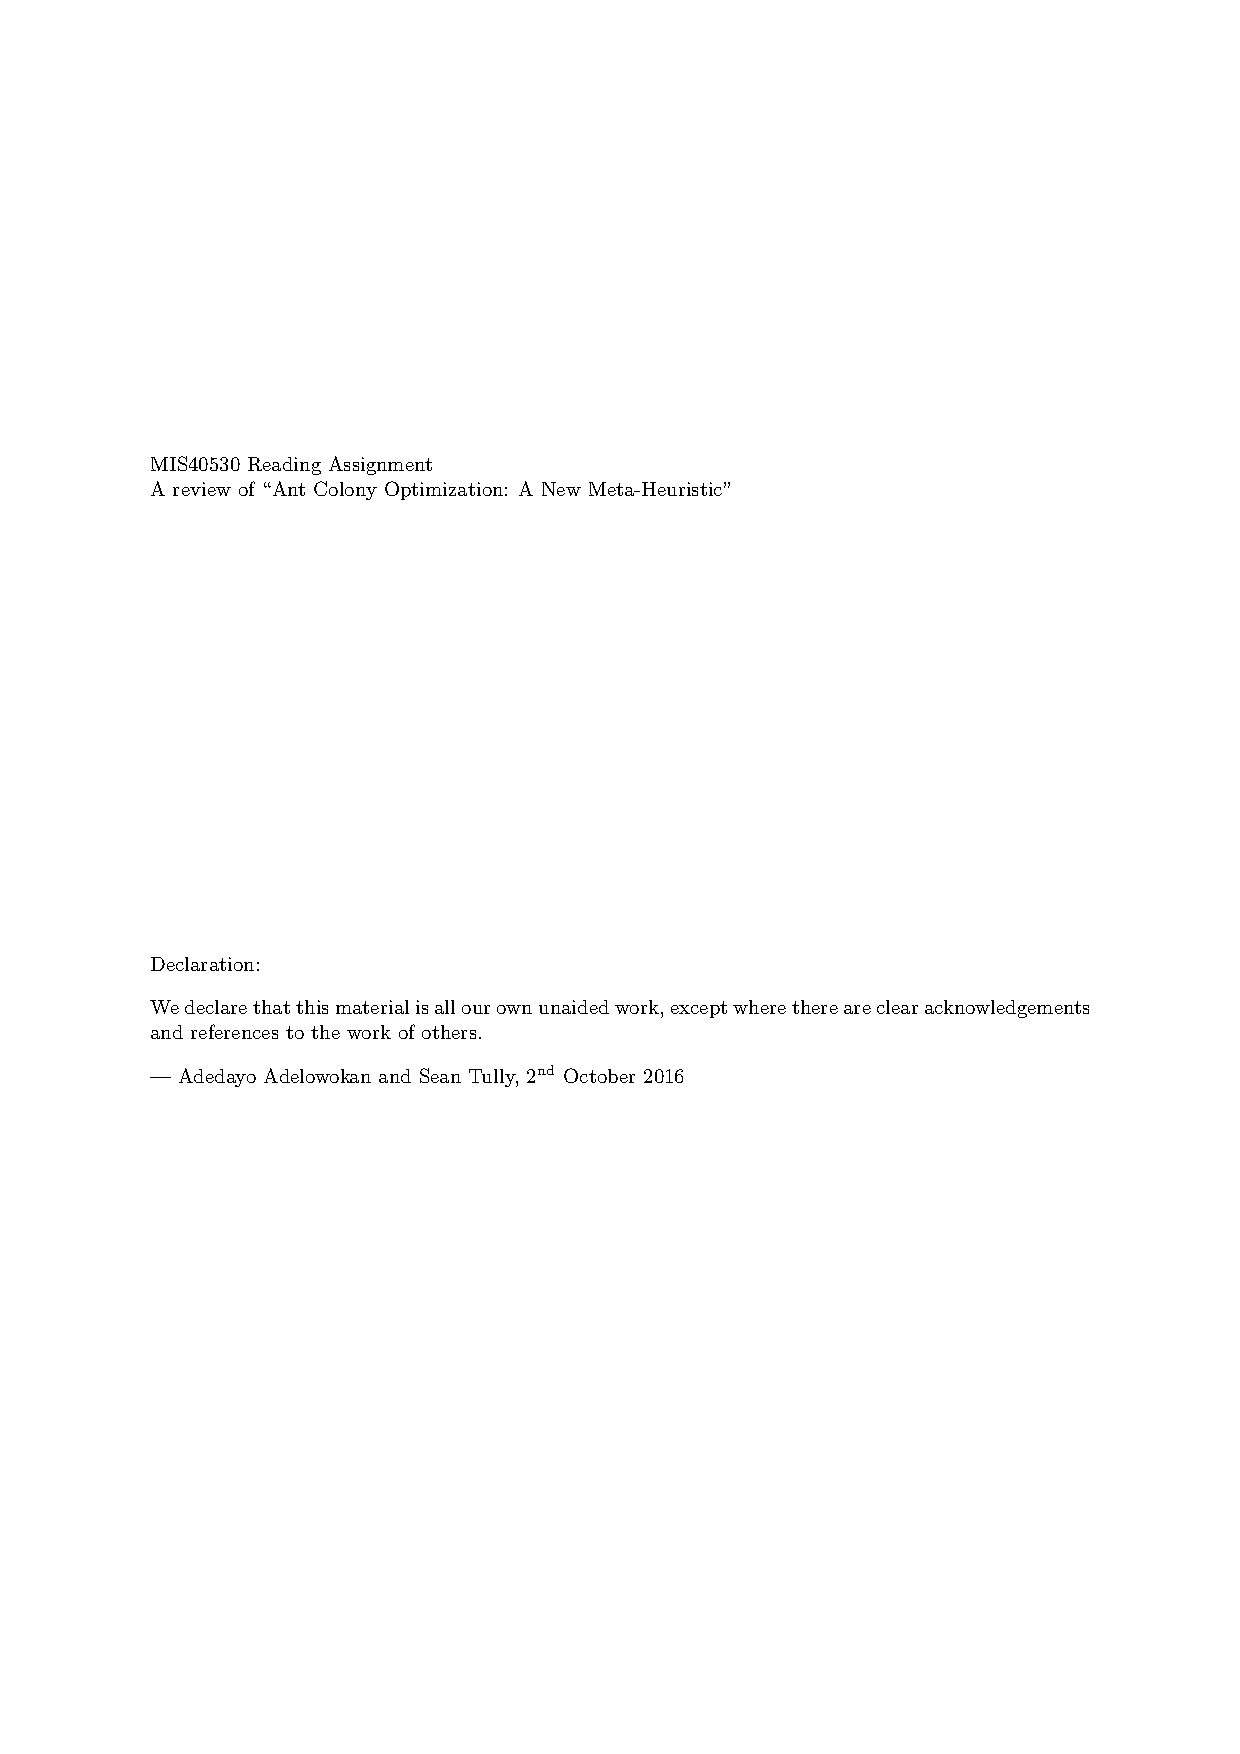
\includepdf{./cover/cover.pdf}
\title{MIS40530 Reading Assignment
\\A review of ``Ant Colony Optimization: A New Meta-Heuristic''}
\author{Adedayo Adelowokan 15204151 MSc(BA) PT\\ Sean Tully 15205062 MSc(BA) PT}
\date{Date of Submission: 2\textsuperscript{nd} October 2016}
\maketitle
The aim of the paper\textsuperscript{*} under review is to provide an overview of ongoing research into algorithms inspired by the behavior of ant colonies and to describe a new meta-heuristic, \emph{Ant Colony Optimization} (ACO), through which these algorithms may be evaluated.  One of the authors, Dorigo, was the instigator of work in this field.  His PhD. thesis, published in 1991, introduced the \emph{Ant System} (AS) heuristic. The paper mentions further work, by Dorigo and by others, which has refined and adapted the original AS concept and applied similar algorithms to a range of discrete optimisation problems.  

The paper does not identify a gap in the research to date \emph{per se}, rather it seeks to refine the characterisation of existing techniques by viewing them through the lens of a new meta-heuristic.

The authors' stated aims are that the ACO meta-heuristic may be used to characterise ongoing work in the field and, furthermore, be useful as a framework for comparing and contrasting such work.  The paper may therefore be viewed as a sort of meta-analysis of existing algorithms; seeking to add to insights gained from existing work in the field.  The authors hope that adoption of the meta-heuristic as a framework in future research will aid ease of development.

The Ant Colony Optimization (ACO) meta-heuristic is introduced as a means of comparing various advances on Dorigo's AS heuristic under a common framework.  The parameters governing a generalised problem and solution are first defined.  A set of rules are defined, governing the behaviour of the ants and an algorithm for the meta-heuristic is presented as pseudocode.  The paper does not describe the solution of a particular problem, but rather introduces two examples of how the meta-heursitic may be applied to solve common discrete optimization problems \emph{viz.} the traveling salesman problem and the problem of routing in communications networks.  The work done in this paper is primarily descriptive; it does not aim to apply a specific algorithm to data nor does it aim to obtain quantitative results.
 
Two applications of the ACO meta-heuristic are explored; the traveling salesman problem and the problem of routing in communications networks.  These applications show that the meta-heuristic provides a suitable framework for categorising problems in the field.  The paper reports success by others in applying similar algorithms to \emph{e.g.} the traveling salesman problem, the quadratic assignment problem and the sequential ordering problem; defining success by comparison to other heuristics.  It should be noted that the success of these algorithms is not predicated on the introduction of the ACO meta-heuristic as a concept, as they predate its introduction.  The paper also highlights applications, such as the job scheduling problem, where related algorithms are not currently competitive with other state-of-the-art techniques. Any results mentioned are qualitative re-statements of the results of others.

The paper seeks to outline the ACO meta-heuristic in a summary fashion and to appraise the reader of current trends regarding various algorithms that may be viewed as applications thereof. The results of others are presented qualitatively, indicating that some algorithms, as implementations of the meta-heuristic, have had success when applied to various discrete optimisation problems.  These results are presented to highlight the usefulness of the meta-heuristic.  

In critiquing the paper, its context must be borne in mind.  It exists as an ``in proceedings'' paper, to inform the reader of the current trends, successes and research in algorithms that may be seen as derivatives of the ACO meta-heuristic.  In this respect, it has achieved these aims. The description of the ACO meta-heuristic was clear and concise and the included pseudocode served as a good illustration of how it may be implemented. The included examples served as a helpful illustration. One criticism is that the authors describe various ``successful implementations of the ACO meta-heuristic''; this may give the impression that the implementations were successful \emph{because} they could be viewed as being derived from the ACO meta-heuristic. Success of the ACO meta-heuristic as a method of characterisation cannot be inferred thus. The ACO meta-heuristic may be deemed a successful characterisation tool if it is both applicable to a wide range of algroithms in the ant colony genre and if it proves to be a relevant and useful tool in the future.  Some evidence of the former was provided in the authors' application of ACO to two problems but the latter can only be borne out with hindsight.  The IEEE currently list 348 citations for the paper (see \url{http://ieeexplore.ieee.org/document/782657/}).  Note that the ACO meta-heuristic was introduced in far more detail in another paper by Dorigo, Di Caro and Gambardella which was also published in 1999, as a peer-reviewed journal paper (\href{https://doi.org/10.1162/106454699568728}{doi:10.1162/106454699568728}); this paper has 3135 citations to date on Google Scholar, which may be viewed qualitatively as validation of the usefulness of the ACO meta-heuristic.
	
\vspace{0.25in}
\noindent
\textsuperscript{*}Dorigo, M. and G. D. Caro, 1999. Ant colony optimization: a new meta-heuristic. In: \emph{Proceedings of the 1999 Congress on Evolutionary Computation}, 1999, volume 2, page 1477. \\doi:10.1109/CEC.1999.782657.

\end{document}
